% 編集した箇所
% 5.1機能概要、5.2前提条件、5.3制約事項、6.1人の流れ、7.想定する利用者

% 編集する必要がある箇所
% 1.はじめに、2.解決できる経営課題、3.課題解決のための提案、4.課題解決のための方法、6.2データの流れ、9.システムのハードウェア構成、15.1費用、15.2効果、16.アピールポイント、17.用語定義

% データの流れ:らず端末のときにログインできないけど、どうやってユーザ登録とかログインするの?
\documentclass[a4j,titlepage]{ujarticle}
\usepackage[dvipdfmx]{graphicx}
\usepackage{enumerate}
\usepackage{url}
\usepackage{listings}


\title{
{ローカル授業支援システム
\\
システム提案書}
\author{\\
\\
\\
\\
\\
Outing Corporation}
\date{\today}
}

\begin{document}
\maketitle


\tableofcontents

\clearpage

\section{サービス利用までの流れ}
\subsection{人の流れ}
このシステムの利用者は、管理者と授業を受ける学生の二通りとなります。

管理者は、スマートフォンやパソコン等の端末から、システム管理者として管理者用のwebページにログインします。
管理者用のホームページからは、学生が使用する端末で表示される進捗管理画面の作成ページ、授業時にリアルタイムで学生から送信されたデータを閲覧できるページ、データベースに蓄積された、過去の学生が送信したデータを閲覧できるページ、データベースの編集ページに遷移することができます。

進捗管理画面の作成を行うページでは、チェックボックスやボタン、フォーム等の用意されたパーツを組み合わせ、配置し、文章の入力を行うことで進捗管理画面の作成を行えます。ここでは、あらかじめシステムに用意された進捗管理画面のレイアウトの雛形を利用することができます。このレイアウトの雛形に進捗や質問、アンケート等の文章を入力することで簡単に画面の作成が行えます。作成した画面のレイアウト及び文章は保存されるため、編集することができます。

作成した進捗管理画面は、授業時に学生の端末に表示させて利用します。学生はスマートフォンまたはRaspberry pi端末からシステムにログイン後、表示された画面の指示に従って、授業時に提示された課題やそれに対する質問、回答を端末に入力し、送信します。学生がデータを送信するたびに、データ閲覧ページは更新されるため、管理者はリアルタイムで学生の入力状況を把握することができます。

また、管理者は、授業時に学生から送信されたデータをいつでも閲覧することができます。


%学生側は、各グループの代表一人が、そのシステムにログインします。
%そして、課題を行う中で進捗状況や質問を入力していきます。
%管理者側は、入力された情報を確認し、実験を円滑に進めます。

システムの運用・保守については管理者が行い、質問等のデータベースの編集も行うことができます。
障害が発生した場合は、システムの再起動を行うことで前回更新した状況まで戻すことで対応します。 % 例えばどんな障害?システム自体の再起動かアプリだけの再起動か?
\begin{figure}[h]

\centering
   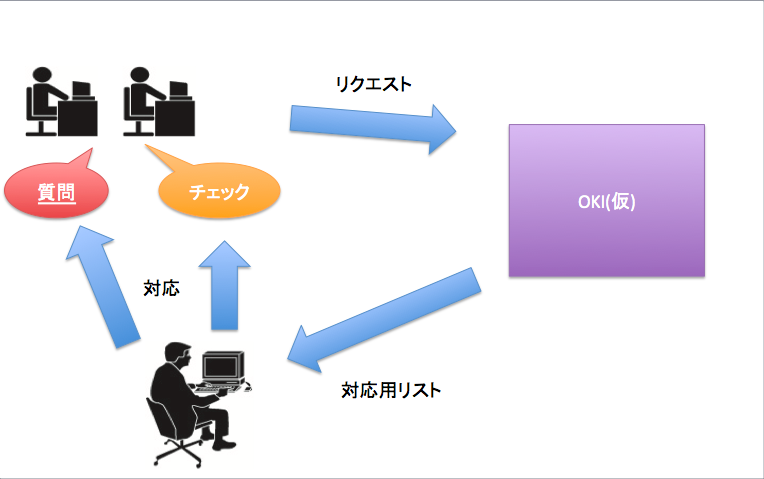
\includegraphics[width=13cm]{hito.png}
  \caption{主な流れ}
\end{figure}


\subsection{データの流れ}
このシステムを利用する際は、はじめにログイン画面が表示され、管理者と学生側とが区別されます。これによってその後画面に表示される内容が変わります。

サーバには管理者が作成した、学生側に表示する画面の情報や質問の情報、課題の進捗状況などが格納されています。学生側には管理者が作成した授業ごとの画面が表示され、学生側が送信した質問内容や進捗状況は管理者がいつでも閲覧できるようになります。また、管理者が質問に対して回答を行うと、その内容がデータベースに蓄積されます。このデータベースの情報から過去の質問内容の確認が行えます。
%このシステムは、ログイン画面によって管理者側と学生側の区別が行われます。そのため、システム自体は同様のものとなり、それとは別にサーバが % 学生側を利用者という言い方は良くない。ログイン画面で区別とは?システム自体が同様を別の言い方で
%存在することでこのシステムの構成要素となります。
%システム内部での情報の流れは以下の図2のようになっています。 % どんな図作る?

%サーバには学生側が登録の際に入力した個人情報や、質問の情報、課題の進捗状況などが格納されています。管理者は終了した講義の情報や次回の講義の
%課題の情報を管理でき、利用者が前提条件に当てはまらなくなった場合には、登録の削除を行うことができます。
\begin{figure}[h]
  \begin{center}
    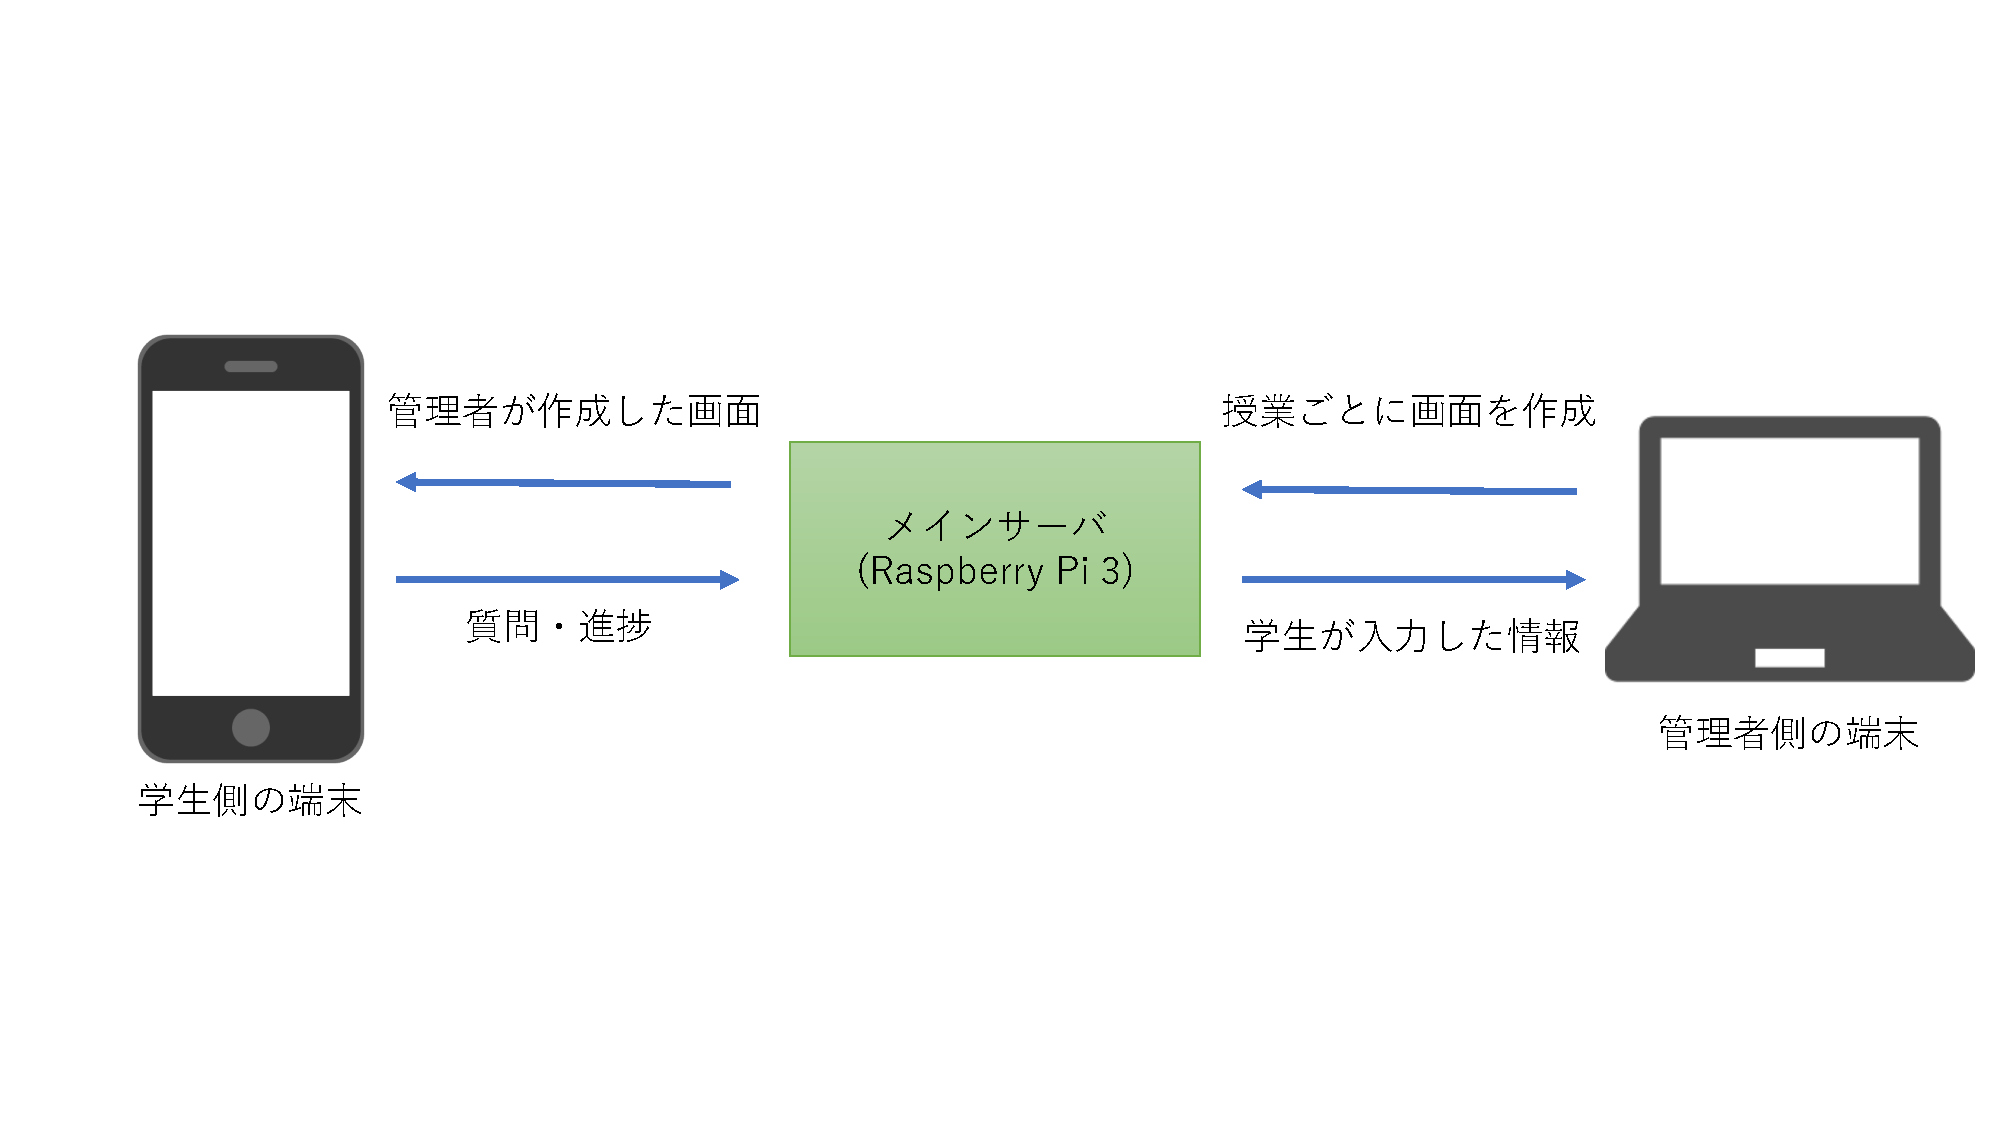
\includegraphics[width=14cm]{data.pdf}
    \caption{データの流れ}
  \end{center}
\end{figure}

%また、質問の一覧のデータを確認、削除することができ、そのデータベースの管理は管理者画面から行うことができます。


\newpage

\end{document}
